\documentclass[a4paper,10pt,twocolumn,oneside,openright,final]{memoir}
\usepackage[english]{babel}
\usepackage{etex}
\usepackage{times}
\usepackage{setspace}
\usepackage{inputenc}
\usepackage{amssymb}
\usepackage{amsfonts}
\usepackage[pdftex]{graphicx}
%\usepackage{subfigure}
\usepackage{alltt}
\usepackage{moreverb}
%for more info on hyperref package see http://en.wikibooks.org/wiki/LaTeX/Packages/Hyperref
\usepackage[pdftex,colorlinks=true,linkcolor=blue]{hyperref}
\usepackage{eso-pic}
\usepackage{transparent}
\setlength{\columnsep}{3em}

\usepackage{wrapfig}
\usepackage{subfig}
\usepackage{alltt}
\usepackage{moreverb}
% tikz related packages to provide scalable graphics 
\usepackage{tikz}
\usetikzlibrary{calc,mindmap,backgrounds,positioning,arrows,shapes,shapes.arrows,shapes.misc,automata,petri,patterns,scopes,chains,matrix,decorations.pathmorphing,shadows,calc}


\usepackage{geometry}
\geometry{hmargin={15mm,15mm},vmargin={15mm,20mm}}

\usepackage[pages=some]{background}

\backgroundsetup{
  scale=1.2,
  angle=0,
  opacity=0.4,
  contents={
    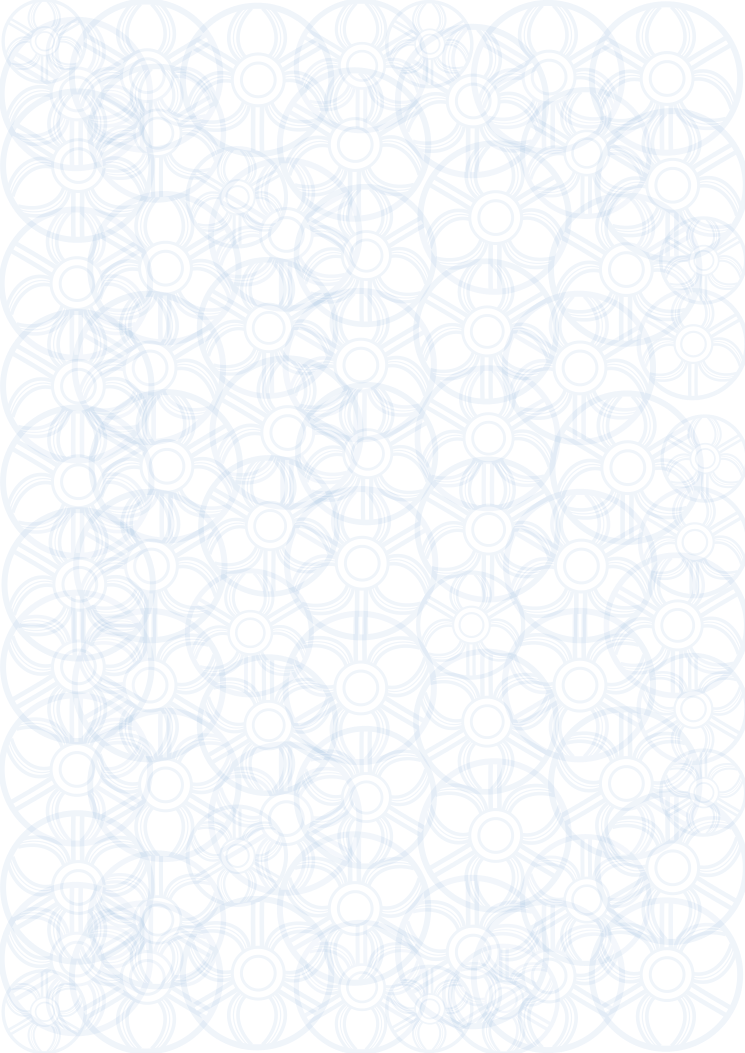
\includegraphics[width=1.1\paperwidth,height=1.1\paperheight, keepaspectratio]{images/00-background.png}} 
}


%%%%%%%%%%%%% copyright %%%%%%%%%%%%%%
\title{Trident Genesis Platform}
\author{Fielden Management Services Europe LLC}
\usepackage{hyperref}
\usepackage{hyperxmp}
\hypersetup{
    pdftitle={Trident Genesis Platform},
    pdfauthor={Fielden Management Services Europe LLC},
    pdfsubject={A hight level overview of key principles and advantages.},
    pdfcopyright={Copyright (C) 2016 by Fielden Management Services Pty Ltd.  All rights reserved.}
}

\usepackage{xcolor}
\makeevenhead{headings}%
    {\thepage}{}{\slshape\bookname~\thebook\qquad\partname~\thepart\qquad\leftmark}
    \makeoddfoot{headings}{\slshape\rightmark}{\color{gray}Copyright (C) 2016 by Fielden Management Services Pty Ltd.  All rights reserved.}{\thepage}
	\makeoddhead{headings}{\slshape\rightmark}{}{}


\copypagestyle{headingsnobook}{headings}
\makeevenhead{headingsnobook}{\thepage}{}{\slshape\leftmark}

\begin{document}

%\BgThispage

\subsection*{What is Trident Genesis?}
  Trident Genesis (TG) is an end-to-end software platform for developing business applications in a domain driven way.
  It lifts the level of abstraction up to the modelling of the business domain, while automatically handling low level technical details.
  
  \vspace{3 mm}
  \noindent The architecture of the business domain is often unique. 
  This is what makes companies competitive.
  Capturing the business domain model in a form of a functional software system that facilitates business operations represents the core value for customers.
  
  \vspace{3 mm}
  \noindent The TG platform incorporates over 30 years of experience in delivering Enterprise grade software solutions at a software architecture level.
  It encapsulates the complexity of the low technical details for efficient database communication, concurrent data processing, HTML5 client construction enabling software developers to concentrate on the business domain architecture.

\begin{figure}[!h]
    \vspace{-5pt} 
    \centering    
    \begin{tikzpicture}[node distance=1cm, auto, opacity=0.8, scale=0.7, every node/.style={scale=0.7}]
      \tikzset{
	  mynode/.style={rectangle,rounded corners,draw=black, top color=white, bottom color=blue!50,very thick, inner sep=1em, minimum size=3em, text centered, text=blue!50!black},
	  platform/.style={rectangle,rounded corners,draw=black, top color=white, bottom color=green!50!white,very thick, inner sep=1em, minimum size=3em, text centered, text=green!50!black}
      }  
      \node at (1, 1) [mynode] (ap1) {Application};
      \node at (1.7, 1.7) [mynode] (ap1) {Application};
      \node at (2.4, 2.4) [mynode] (ap1) {Application};

      \def\platformpath{-- +(5cm,0cm) -- +(5cm,2cm) -- +(3cm,2cm) -- +(3cm,2.5cm) -- +(4cm,2.5cm) -- +(2.5cm,3.5cm) -- +(1cm,2.5cm) -- +(2cm,2.5cm) -- +(2cm,2cm) -- +(0cm,2cm) -- cycle}
      \draw (-1,-3.3) [platform] \platformpath 
	    node [below,text width=7em, text centered,xshift=2.2cm,yshift=0.8cm] {Trident Genesis Platform};  
    \end{tikzpicture}
    \vspace{0pt} 
  \end{figure}

  \noindent The typical software construction workflow with TG encompasses: modelling of the business domain (declarative ontological aspect), implementing core business rules (imperative aspect) and configuring the user interface.
  These steps are facilitated by high level abstractions provided by the platform.
  The platform enables developers to concentrate on the modelling of the business domain. 
  This ensures higher productivity, quality and value of the final software system for the business.


 \subsection*{Principles and Advantages}
  	TG is designed to ensure that the application facilitates communication between different business stakeholders and is easy to use by incorporating the following principles and approaches.

\subsubsection*{Unique object-oriented architectural style to uniform modelling of the business domain}
	One could argue that commanding a programming language is relatively easy. 
  	However, object-oriented design is a different story.
  	It takes many years to become an experienced software architect.
  	TG provides a well defined architectural style that not only solves low technical tasks, but most importantly incorporates a unique architectural approach to uniform modelling of the business domain.
  	The platform ensures that all TG-based applications follow exactly the same development and modelling style, which leads to structural and behavioural uniformity of the final software system.
  	This protects developers from a multitude of programming errors.
	It enables agile development of working solutions that can be easily supported by both the original or new developers.

    \begin{figure}[!h]
    %\vspace{20pt}
    \centering    
    \begin{tikzpicture}[>=latex', scale=1.0, every node/.style={scale=1.0}]
      \tikzset{
	  outercore/.style={circle, fill=blue!50!white, inner sep=0em, minimum size=0.6cm},
	  core/.style={circle, shade, ball color=green!50!white, inner sep=0em, minimum size=0.3cm},
	  score/.style={circle, fill=green!50!black, inner sep=0em, minimum size=0.3cm},
	  outer/.style={circle, fill=blue!50!white, inner sep=0em, minimum size=2.3cm},
      }
      \begin{scope}[opacity=0.8]
	\node (o) at (0, -0.25) [outer, opacity=0.3] {};      
	\fill[circle, color=green!50!white] (0, -0.25) circle (0.7cm) node [below,text=blue!50!black,yshift=1.1cm] {Synthesised Domain Entity Model};
      \end{scope}
      
      \begin{scope}[scale=0.3,opacity=0.8]
	\node (t) at (0,0) [outercore, opacity=0.5] {};	
	\node at (0,0) [core, opacity=0.5] {};

	\node (r) at (1,-1.2) [outercore, opacity=0.5] {};	
	\node at (1,-1.2) [core, opacity=0.5] {};

	\node (l) at (-1,-1.2) [outercore, opacity=0.5] {};	
	\node at (-1,-1.2) [score] {};
      \end{scope}
      
      \node (pe) at (1.3, 1.5) [text=green!50!black,scale=0.8] {Persistent Entities};      
      \fill [green!50!black,->,out=-100, in=80] (pe.south) edge (t.north);
      \fill [green!50!black,->,out=-100,in=80] (pe.south) edge (r.north);
      
      \node (se) at (-1.3, 2) [text=blue!50!black,scale=0.8] {Synthesised Entities};
      \fill [blue!50!black,->,out=-60,in=160] (se.south) edge (l.west);
      \fill [blue!50!black,->,out=-80,in=160] (se.south) edge (o.west);      
    \end{tikzpicture} 
    \vspace{-60pt}
  \end{figure}

\subsubsection*{Single programming language (Java)}
	Modern software technology stacks are diverse and complex.
	Separate layers often follow different approaches, and may require different languages to use them.
	Databases require SQL knowledge, constructing Web UI requires the knowledge of HTML, CSS and JavaScript, the middleware requires some other language such as Java, Scala or C\# as well as associated frameworks.
	All of this makes software construction a complex multidisciplinary activity.
	Adding the requirement for proper modelling of the actual business domain on top of that only complicates the situation, which explains why so many software projects do not get completed or fail under their own weight during the maintenance lifecycle.
	That's why one of the core principles of TG is \emph{one language to rule them all}.
	This single language is Java, one of the currently most popular programming languages.
	Application developers that know Java can use TG to concentrate on building a core business value and deliver scalable and responsive software solutions without delving deep into the underlying technology stack.
	The developers continue to use their favourite IDE and take advantage of interactive debugging and static code analysis tools.

\subsubsection*{Optimised for relational databases}
	The TG platform was developed inside-out -- this is the solution we use to deliver high quality EAM/ERP systems to our customers.
	That's why unlike alternative solutions that follow the hype of NoSQL and Object-Relational databases, the TG platform provides optimised integration with relational databases such as Oracle, SQL Server and PostgreSQL.
	It utilises the business domain knowledge from the model in order to dynamically optimise queries and adjust to data usage patterns at runtime.
	Instead of using SQL, which does not fit well into the object-oriented thinking, the platform provides Entity Query Language, which is an embedded domain specific language that allows expressing data queries in a natural manner for object-oriented models by traversing the object graph.

\subsubsection*{Automated business domain model verification by means of domain driven testing}
	The notion of automated testing is frequently used to ensure the quality of software systems.
	Unfortunately, often unit and functional testing is an afterthought and software technology stacks need to be expanded with additional facilities to enable such testing, and these do not necessarily fit well with the rest of the layers.
	The TG platform provides first-class support for unit and functional testing in a domain driven way.
	Tests get specified against the developed business domain model by using that model.
	Unit and functional tests represent verification rules and the provided domain driven testing approach ensures their evolution alongside the underlying business domain model.
	This makes Test Driven Development (TDD) a natural approach to developing software systems with TG.
	
\subsubsection*{Continuous validation and integration of the business domain models during the system lifecycle}
	The TG platform stands on the shoulders of giants.
	This is no different when it comes to continuous integration (CI) and validation of TG-based software systems.
	The domain driven testing is fully compatible with modern CI tools like Jenkins and Hudson.
	Thus, the systems lifecycle can be fully integrated with one of CI tools to ensure continuous validation of the business domain model underpinning the software system.

\subsubsection*{Direct interaction and manipulation of the business domain model}
	The worldview metaphor is fundamental to the TG platform, where the \emph{world} is an actual business domain model.
	This means that software developers and the end system users have direct access to the same model!
	While developers interact with the model at the code level and can enhance it, the system users can interact with and manipulate exactly the same model through UI.
	Users can review business entities, their relationships, enhance them with calculated properties from UI for the purpose of data interrogation, analysis and reporting.
	This significantly reduces the misconceptions about the system's actions, structure and logic, and empowers the users to truly utilise the capabilities of the business domain model to its fullest potential.
	Instead of using external tools for accessing raw data in underlying databases, the users are provided with an embedded business intelligence capability to interact with the data through a well defined business domain model.
	\begin{figure}[!h]
  		\centering
  		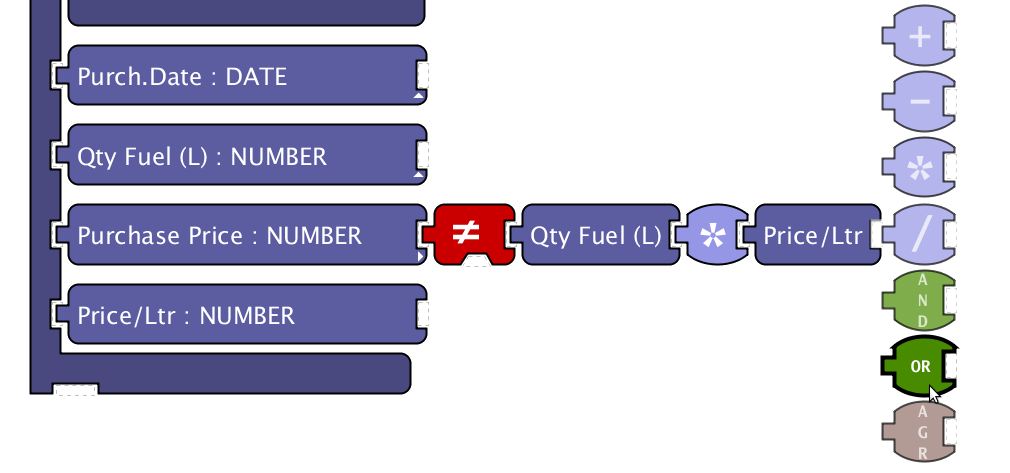
\includegraphics[scale=0.20]{images/01-rulesarea-suggestionmenu.png}  
		\vspace{-30pt} 
  	\end{figure}

%\BgThispage

\subsubsection*{Responsive HTML5 clients}
	TG employs an internal domain specific language for defining responsive Web UI.
	The UI concepts are all based on the business domain modelling principles to reinforce the worldview metaphor, and follow the Google Material Design spec to deliver responsive and consistent User Experience (UX) across devices of multiple form factors.
	The TG presentation layer is based on Web Components (built with Google Polymer), which enables reuse and integration of in-house and $3^{rd}$ party components.
	TG offers a search-first approach to UX design that provides users with sophisticated first-class data retrieval tools supporting model-driven selection criteria, value autocompletion, ranges, meta-conditions (e.g. missing value, this year, previous fortnight), aggregations and sorting of the result sets. 

	
\subsubsection*{A software construction tool to facilitate the process management}
	Agile, Kanban, Scrum, FDD, TDD\ldots all of these and more are the management techniques, methodologies and methods to ensure the development of high quality and timely delivered software systems.
	These project management approaches exist for a good reason and there are multiple tools that assist with their implementation and practicing.
	This, however, is only one side of the coin.
	Implementing a proper process management method does not solve the software construction problem.
	It does not take away the technical needs and issues that arise during software construction.
	It can only help in mitigating them.
	That's why having an appropriate software construction tool that works well together with the process management method is vital to the success of any software project.
	Using the TG platform elevates software developers to the business domain level, establishes a ubiquitous business domain specific language to facilitate communication between the project stakeholders.


\subsubsection*{Robust Security}
	Industrial grade security, which includes HTTPS communication, the use of a key stretching PBKDF2 based password hashing, mutating session authenticator strategy, reduced sign-on with the support of both trusted and untrusted devices. 
	Support for multi-factor authentication scheme. 
	Declarative authorisation with pluggable backends (e.g. LDAP).

    
    
\subsubsection*{Cloud ready}
	Software systems built with TG are cloud ready.
	The platform employs RESTful architecture to structure application web-resources.
	This ensures clean separation between different business domain boundaries, UI resources and provides excellent capacity for scalability.

\subsubsection*{Complete application development lifecycle}
	One of the key meta-features of the Trident Genesis platform is its ability to support a complete lifecycle for developing software systems.
	This was one of our essential goals.
	Otherwise, there would always be low level technical aspects to software development that interrupt high level business domain oriented developer thinking.
	Thus, the development of software systems with TG covers all that is required for end-to-end software construction.
	This includes orthogonal aspects such as unit and functional testing, build and installation, business model design and database integration, UI definitions, secure HTTP communication, scalability and more.

\end{document}

